\FloatBarrier
\section{Weiterführende Abbildungen}
\subsubsection{Umfrageergebnis}
\begin{figure}
\centering
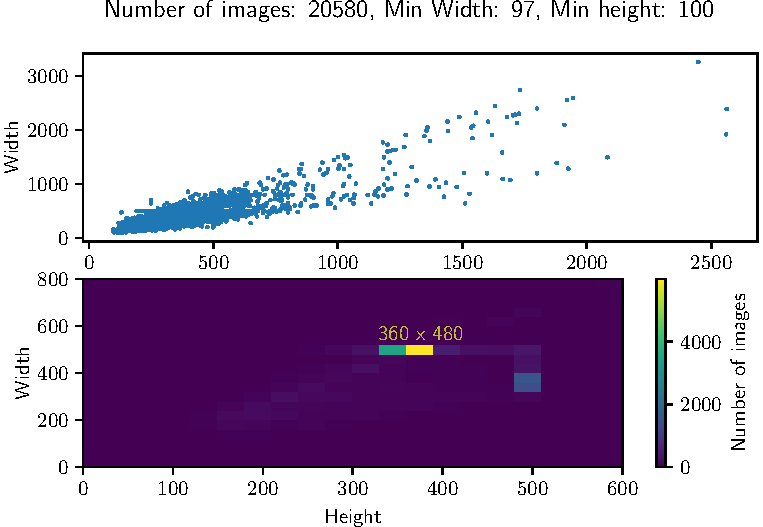
\includegraphics[width=\the\textwidth]{../../final_data/MiniNN_n120/width_heigt_scatter_hist2d.pdf}
\caption{Oben: Scatter-Plot der Höhen- und Breitenverteilung der Bilder aus dem
großen Datensatz. Unten: Zweidimensionales Histogramm der Höhen- und Breiten-
verteilung. Die gelbe Größe entspricht der am häufigsten auftretenden Kombination
aus Breite und Höhe.}
\label{fig:Bildverteilung_Datensatz}
\end{figure}
\begin{figure}
\centering
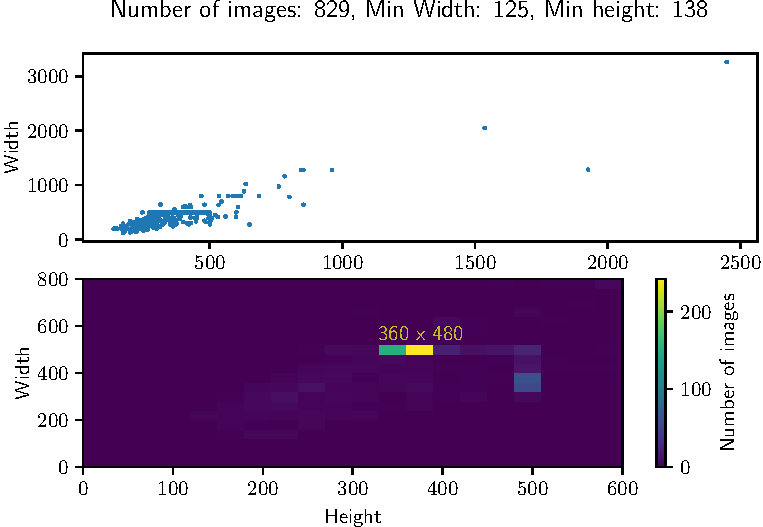
\includegraphics[width=\the\textwidth]{../../final_data/MiniNN_n5/width_heigt_scatter_hist2d.pdf}
\caption{Oben: Scatter-Plot der Höhen- und Breitenverteilung der Bilder aus dem
kleinen Datensatz. Unten: Zweidimensionales Histogramm der Höhen- und Breiten-
verteilung. Die gelbe Größe entspricht der am häufigsten auftretenden Kombination
aus Breite und Höhe.}
\label{fig:Bildverteilung_Datensatz_MiniDataset}
\end{figure}
\FloatBarrier
\FloatBarrier
\subsection{Bildgrößenverteilung}
\begin{figure}
\centering
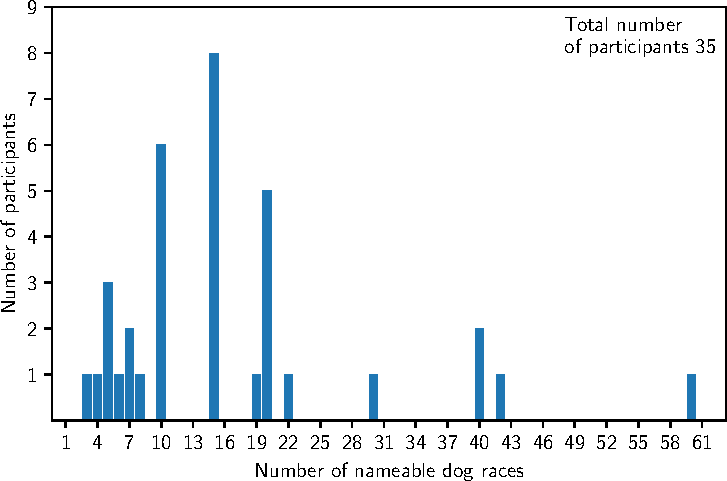
\includegraphics[width=\the\textwidth]{./survey/answers_plot.pdf}
\caption{Antwortverteilung der Umfrage unter Physikstudierenden.}
\label{fig:Antwortverteilung}
\end{figure}
\FloatBarrier
\subsubsection{Beispielhafte Netzarchitektur}
\FloatBarrier
\begin{figure}
\centering
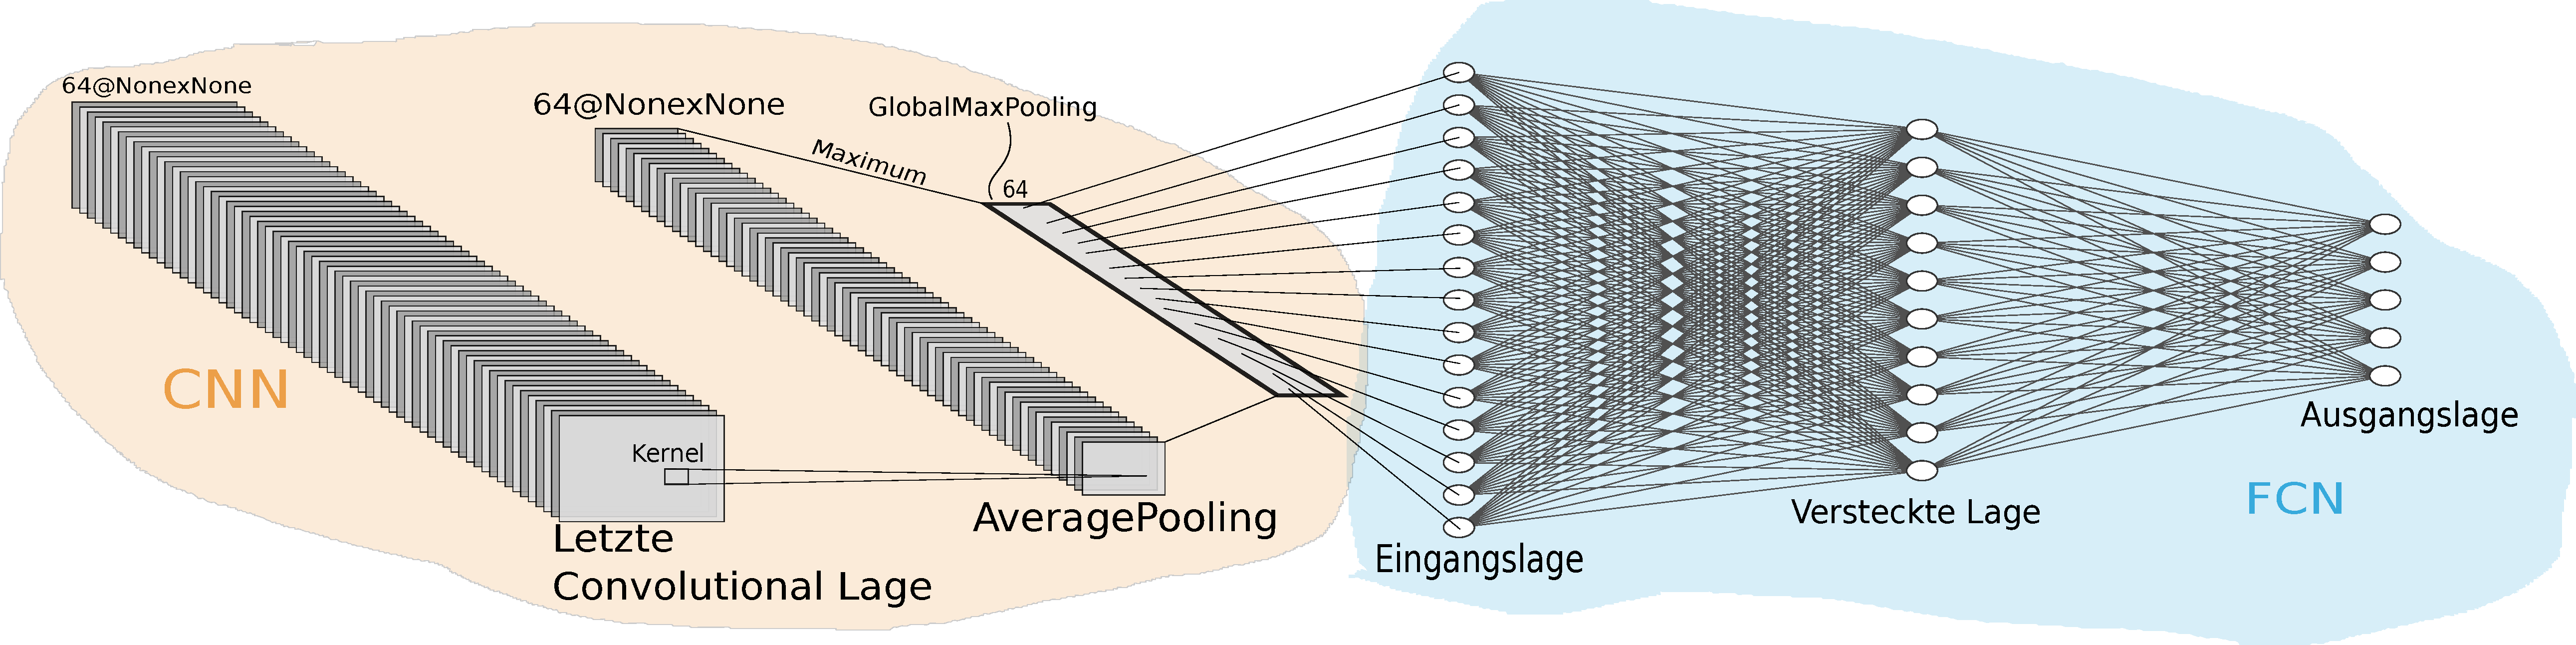
\includegraphics[width=\the\textwidth]{../../final_data/general/sample_network.pdf}
\caption{Schmatische Darstellung der verwendeten Architektur, wobei
         die Aktivierungsfunktionen nicht mit eingezeichnet sind. Erläuterung der Konvention: \emph{\textbf{\#}Filter\textbf{@}Bildbreite \textbf{X} Bildhöhe}.
         Die Grafik wurde unter zuhilfe nahme der Internetseite \cite{net_svg_source} erstellt.}
\label{fig:beispielhafte_netz_architecture}
\end{figure}
\FloatBarrier
\subsubsection{Ergebnisse MiniDogNN für $120$ Hunderassen}
\FloatBarrier
\begin{figure}
\centering
\centering
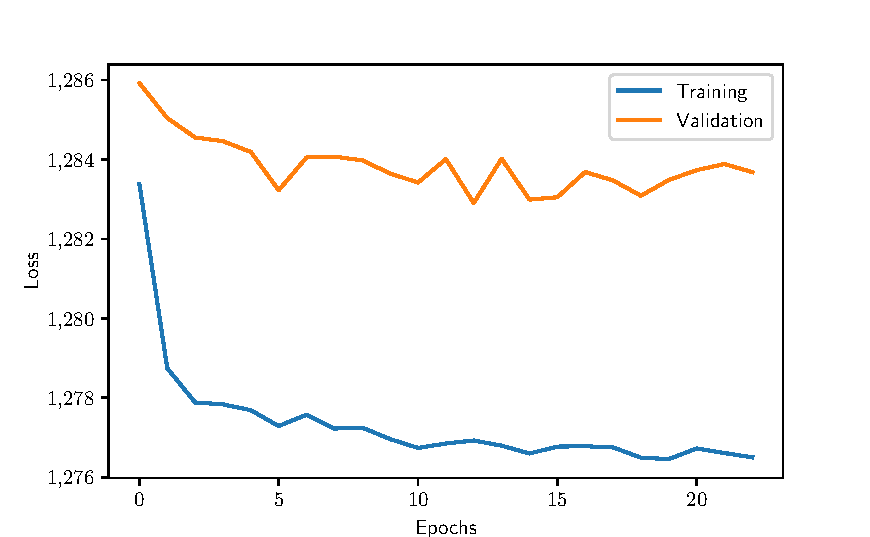
\includegraphics[width = \textwidth]{../../final_data/MiniNN_n120/08-07-2019_21:08:09_n_120/build/history_loss.pdf}
\caption{Traningsfortschritt des \textsc{MiniDogNN}.}
\label{fig:MiniDogNN_120_Loss_Acc}
\end{figure}
\begin{figure}
\centering
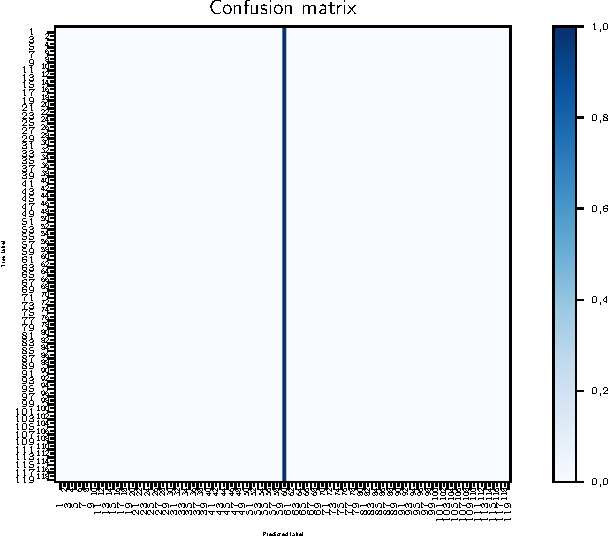
\includegraphics[width = 0.8\textwidth]{../../final_data/MiniNN_n120/08-07-2019_21:08:09_n_120/build/confusion_matrix.pdf}
\caption{Konfusionmatrix des \textsc{MiniDogNN}.}
\label{fig:MiniDogNN_120_Konfusionmatrix}
\end{figure}
\FloatBarrier
\subsubsection{Genauigkeitverteilung MiniDogNN}
\FloatBarrier
\begin{figure}
\centering
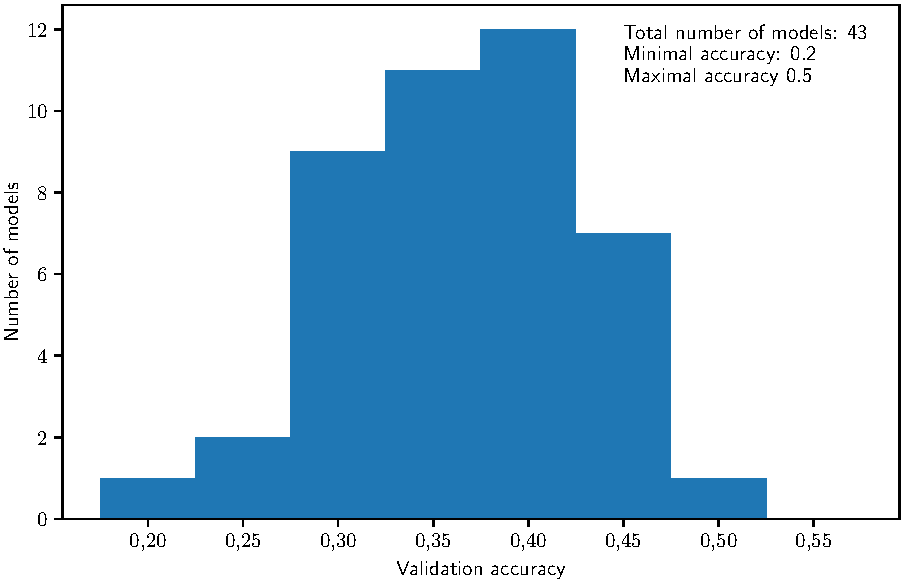
\includegraphics[width=\the\textwidth]{../../final_data/MiniNN_n5/acc_hist.pdf}
\caption{Genauigkeitverteilung der erfolgreich tranierten Modelle der HPO.}
\label{fig:Genauigkeitverteilung_MiniDogNN}
\end{figure}
\subsubsection{Legende}
\begin{table}
	\centering
	\caption{Legende für die Confusion-Matrizen des großen Datensatzes (Teil 1)}
	\label{tab:legende_rf}
	\begin{tabular}{c l | c l}
	\toprule
		{Label} &
		{Hunderasse} & {Label} &
		{Hunderasse} \\
	\midrule
		 1 & Afghan hound & 31 & Great Pyrenees \\
		 2 & African hunting dog & 32 & Greater Swiss Mountain dog \\
		 3 & Airedale & 33 & Ibizan hound \\
		 4 & American Staffordshire terrier & 34 & Irish setter \\
		 5 & Appenzeller & 35 & Irish terrier \\
		 6 & Australian terrier & 36 & Irish water spaniel \\
		 7 & Bedlington terrier & 37 & Irish wolfhound \\
		 8 & Bernese mountain dog & 38 & Italian greyhound \\
		 9 & Blenheim spaniel & 39 & Japanese spaniel \\
		 10 & Border collie & 40 & Kerry terrier \\
		 11 & Border terrier & 41 & Labrador retriever \\
		 12 & Boston bull & 42 & Lakeland terrier \\
		 13 & Bouvier des Flandres & 43 & Leonberg \\
		 14 & Brabancon griffon & 44 & Lhasa \\
		 15 & Brittany spaniel & 45 & Maltese dog \\
		 16 & Cardigan & 46 & Mexican hairless \\
		 17 & Chesapeake Bay retriever & 47 & Newfoundland \\
		 18 & Chihuahua & 48 & Norfolk terrier \\
		 19 & Dandie Dinmont & 49 & Norwegian elkhound \\
		 20 & Doberman & 50 & Norwich terrier \\
		 21 & English foxhound & 51 & Old English sheepdog \\
		 22 & English setter & 52 & Pekinese \\
		 23 & English springer & 53 & Pembroke \\
		 24 & EntleBucher & 54 & Pomeranian \\
		 25 & Eskimo dog & 55 & Rhodesian ridgeback \\
		 26 & French bulldog & 56 & Rottweiler \\
		 27 & German shepherd & 57 & Saint Bernard \\
		 28 & German short-haired pointer & 58 & Saluki \\
		 29 & Gordon setter & 59 & Samoyed \\
		 30 & Great Dane & 60 & Scotch terrier \\
		 \bottomrule
	 	\end{tabular}
	 \end{table}

	 \begin{table}
	 	\centering
	 	\caption{Legende für die Confusion-Matrizen des großen Datensatzes (Teil 2)}
	 	\label{tab:legende_rf_2}
	  \begin{tabular}{c l | c l}
	 	\toprule
		{Label} &
		{Hunderasse} & {Label} &
		{Hunderasse} \\
	 	\midrule
		 61 & Scottish deerhound & 91 & curly-coated retriever \\
		 62 & Sealyham terrier & 92 & dhole \\
		 63 & Shetland sheepdog & 93 & dingo \\
		 64 & Shih-Tzu & 94 & flat-coated retriever \\
		 65 & Siberian husky & 95 & giant schnauzer \\
		 66 & Staffordshire bullterrier & 96 & golden retriever \\
		 67 & Sussex spaniel & 97 & groenendael \\
		 68 & Tibetan mastiff & 98 & keeshond \\
		 69 & Tibetan terrier & 99 & kelpie \\
		 70 & Walker hound & 100 & komondor \\
		 71 & Weimaraner & 101 & kuvasz \\
		 72 & Welsh springer spaniel & 102 & malamute \\
		 73 & West Highland white terrier & 103 & malinois \\
		 74 & Yorkshire terrier & 104 & miniature pinscher \\
		 75 & affenpinscher & 105 & miniature poodle \\
		 76 & basenji & 106 & miniature schnauzer \\
		 77 & basset & 107 & otterhound \\
		 78 & beagle & 108 & papillon \\
		 79 & black-and-tan coonhound & 109 & pug \\
		 80 & bloodhound & 110 & redbone \\
		 81 & bluetick & 111 & schipperke \\
		 82 & borzoi & 112 & silky terrier \\
		 83 & boxer & 113 & soft-coated wheaten terrier \\
		 84 & briard & 114 & standard  poodle \\
		 85 & bull mastiff & 115 & standard schnauzer \\
		 86 & cairn & 116 & toy poodle \\
		 87 & chow & 117 & toy terrier \\
		 88 & clumber & 118 & vizsla \\
		 89 & cocker spaniel & 119 & whippet \\
		 90 & collie & 120 & wire-haired fox terrier \\
	\bottomrule
	\end{tabular}
\end{table}

\FloatBarrier
\subsubsection{Traningsdokumentation Autoencoder}
\FloatBarrier
\begin{figure}
\centering
\centering
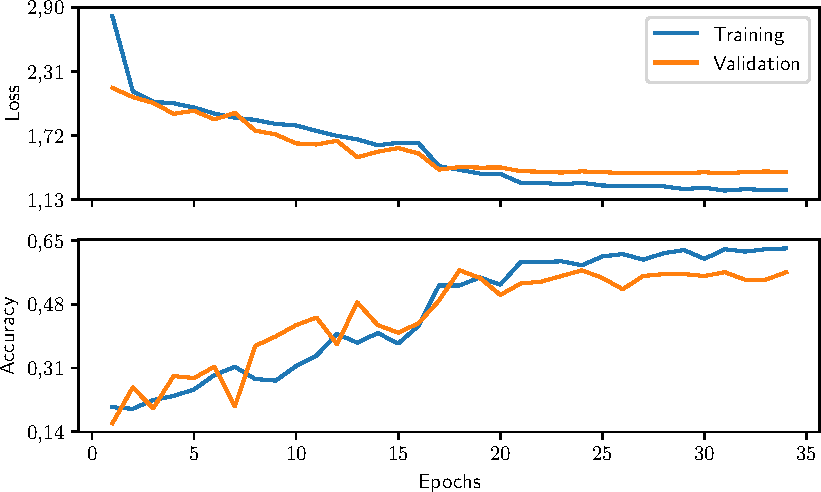
\includegraphics[width = \textwidth]{../../final_data/autoencoder_n_120/build/history.pdf}
\caption{Traningsfortschritt des Autoencoders.}
\label{fig:Autoencoder_loss}
\end{figure}
\FloatBarrier

\subsubsection{HPO des Randomforests}
\FloatBarrier
Paramterraum für die HPO:
\begin{align}
  \begin{aligned}
    \label{eq: rf_parameter_raum}
    max_d &\in \left\{\infty,\, 10,\, 100\right\} & n\ua{feat}&\in\left\{auto, \,log2\right\}\\
    min\ua{leaf} &\in \left\{1,\, 10,\, 31\right\} & min\ua{split}&\in\left\{2,\, 8,\, 10\right\}\\
    crit &\in \left\{gini,\, entropy\right\} & n\ua{est}&\in\left\{100,\, 400,\, 1000,\, 1500 \right\}
  \end{aligned}
\end{align}
\FloatBarrier
